\documentclass[11pt,twocolumn]{article}
\usepackage[utf8]{inputenc}
\usepackage{graphicx}
\usepackage{color}
\usepackage[margin=1.in]{geometry}
\usepackage{wrapfig}
\usepackage[utf8]{inputenc}
\usepackage{longtable}
\setcounter{page}{3}

\begin{document}
\begin{titlepage}
\centering
	
\includegraphics[width=0.30\textwidth]{logo.png}\par\vspace{1cm}
	{\scshape\LARGE Massey University \par}
	\vspace{1cm}
	{\scshape\Large Individual Research: 228.798\par}
	\vspace{1.5cm}
	{\huge\bfseries Literature Review \par}
    \vspace{1cm}
    {\large\bfseries Self morphing soft robotic gripper for the handling and manipulation of delicate produce in horticultural applications\par}
	\vspace{2cm}
	{\large\itshape Dean Gerhardus Venter\par}
	\vspace{2cm}
	{\large\itshape 14074740\par}
	\vfill
	supervised by\par
	Dr. Steven  \textsc{Dirven}
   
	\vfill

% Bottom of the page
	{\large \today \par}
\end{titlepage}
\title{Abstract}
\maketitle
\noindent
The following literature review is based on the current and past methods of robotic gripping with a focus on soft robotics. The purpose of the research is to deduce the optimal gripping method to grip soft and delicate objects, specifically kiwifruit and berries. The kiwifruit industry alone is worth in excess of \$1,181.9 billion dollars \cite{fresh_facts_2015}, however , virtually all of the produce is being picked manually or by soft robotic grippers which are not upto the required efficiency due to damaging the produce during the harvesting phase. The scope of the research is to investigate the current and past gripping methods in order to deduce how each method works and the advantages and disadvantages associated with each of the respective methods. The knowledge which has been acquired will be used in order to guide the development of a novel gripping mechanism which aims to be equally or more efficient than the currently used harvesting methods. The gripping methods which have been investigated are:
\begin{enumerate}
\item Mechanical Gripper
\item Tendon Actuated soft gripper
\item Pneumatic under actuated gripper
\item Particle jamming gripper
\item Electro Active Polymers
\end{enumerate}
From the research which has been done, it is clear o see that there is no perfect gripping mechanism due to each mechanism having their respective advantages and disadvantages. From the research which has been done, the pneumatic under-actuated gripper appears to be the most suitable method amongst the researched techniques. However, aspects of other gripping methods will be taken into consideration when producing a  prototype gripper to work towards producing a optimal gripping mechanism to handle delicate fruit and produce.

\begin{titlepage}
\tableofcontents
\end{titlepage}
\section{Introduction}
The capability to autonomously grasp objects using robotics remains a chalenge, even in the modern day and age since engineers continually strive to produce a controllable gripper which is equally or more effective than the the anthropomorphic hand \cite{bogue2016flexible}. Conventional robotic grippers in past have either been unable to achieve a successful grasp of modular objects due to the feedback sensors required to deduce whether a gripper has been successfull or not whilst not causing any damage to the product during manipulation. There are a wide range of robotic grippers available in industry, all of which have different capabilities and purposes. Conventional grippers are currently prodominantly being produced using rigid links, mechanical joints and are mechanically actuated \cite{ilievski2011soft}. However, the conventional methods are not suitable for delicate operations such as minimally invasive surgery or handling delicate objects such as produce in the form of fesh fruit and vegetables, thus, soft robotics has been becoming an increasingly popular substitute. The research is being done in order to produce soft robots which are capable of completing tasks which conventional rigid-bodied robots are virtually incapable of doing such as delicately handling soft items or working alongside humans \cite{bilodeau2015monolithic}.
\\
\newline
Soft robotics is a biologically inspired class of machinery which is produced using non-rigid, elastomer's which have the capability to morph and conform around the object which they are gripping to varying extents much like how living creatures handle objects.\cite{ilievski2011soft,bilodeau2015monolithic,mosadegh2014pneumatic,martinez2013robotic,marchese2015recipe}. Soft robots are defined as machines made of soft, elastomer type materials or machines composed of multiple hard-robotic actuators that operate in concert, and demonstrates soft-robot-like properties \cite{ilievski2011soft}. The rigidity of the gripper can be altered in order to suit the required application, allowing it to be more compliant and have multiple to an infinate degree of freedom \cite{hassan2015design}. By using soft materials, it allows us to mimic the capability of the soft tissue of animals morphing around the object which is being grasped, thus allowing for the stress being produced in the grasp to be distributed over a larger area, reducing the pressure on the object being grasped \cite{ilievski2011soft}. In the case of grasping delicate objects, this capability is highly sought after because it allows for no point loading, thus reducing the risk of damage  during handling.
\\
\newline
There is a wide range of soft grippers which operate differently based on the geometrical layout of the gripper as well as the actuation. Such grippers include:
\begin{itemize}
\item Mechanically actuated
\item Tendon actuated
\item Pneumatically actuated
\item Particle jamming
\item Electro-Active Polymer  
\end{itemize}
In the following report, each of the different applicable methods will be discussed, exploring the advantages and disadvantages associated with each method in order to deduce an optimal gripping method to be used in the scope of my research problem.
\section{Project Context}
Harvesting fresh produce is a very taxing and labour intensive task, however , currently virtually all of the harvesting of delicate produce, especially kiwifruit and berries is completed manually, whilst some companies are working towards automating the system. Due to the fact that the harvesting is such a taxing and laborious task, finding the staff to efficiently pick and pack the fruit is rather difficult and can lead to losses if the produce is not packed in time or incorrectly. In 2015 the New Zealand horticulture industry estimated the export of fresh and processed fruits to be worth in excess of \$2.14 billion dollars, of which kiwi fruits made up approximately \$1,181.9 billion dollars as shown in Figure \ref{fig:Pie} \cite{fresh_facts_2015}. The New Zealand export industry is of the utmost importance to growth of the local economy, thus it is in the interest of all kiwi's to optimise our exports whether it is dairy, horticultural or meats. In the horticulture industry, a major challenge is to harvest the produce efficiently, especially delicate produce such as kiwi fruit and berries. The current method of harvesting delicate produce is mostly manual seasonal labour as well as a small portion of the industry exploring soft robotic options. However, neither of the two current options which are currently being used for harvesting are meeting the efficiency requirements. The issues associated with the current methods are discussed below:
\begin{figure}[h]
\centering
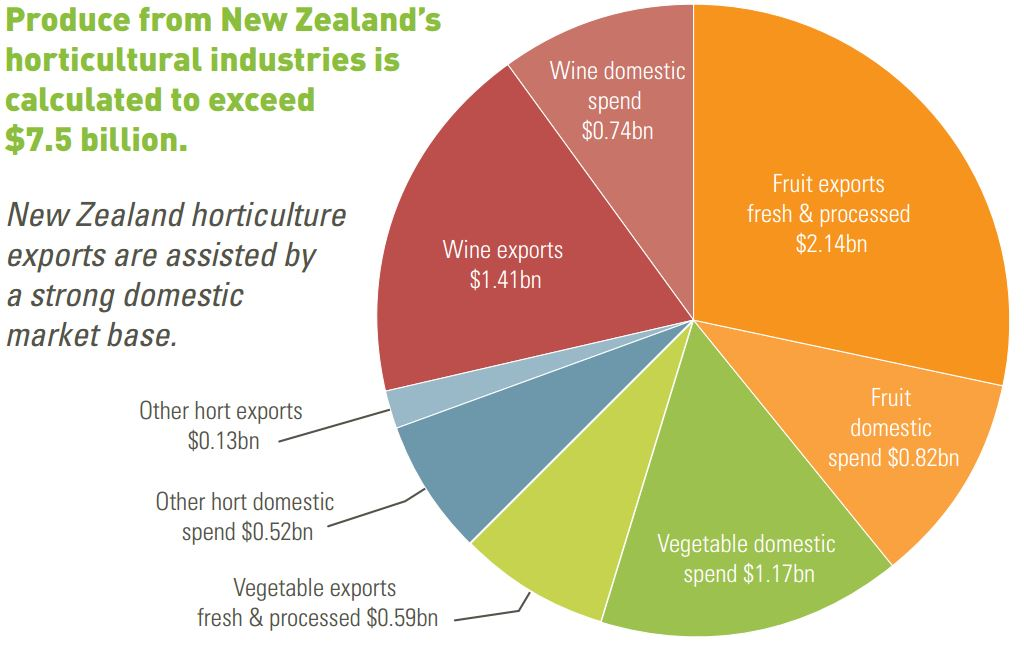
\includegraphics[scale=0.37]{pie_imports}
\caption{New Zealand horticultural exports}
\label{fig:Pie}
\end{figure}
\subsection{Manual seasonal labour}
The kiwi fruit harvesting season in New Zealand is between the months of April and August, meaning that there is not year-round harvesting of the fruits. This is an issue due to the fact that it means that the staff which manually harvest the fruits by hand is mostly comprised of seasonal foreign staff who are working tourists. Thus, virtually no experience can be built by staff, therefore for the initial stages of the harvest, the picking technique is poor, leading to damaged produce and injured staff. In the year dated July 2015 to June 2016, there was a total of 4,084 claims made to the ACC for farm workers who had sustained an injury caused by Lifting and/or carrying objects. This amounted to a total cost of \$7,283,868 to treat \cite{injury_statistics_tool_2017}. A major contributing factor to this is the sheer size of the loads these staff have to carry, causing their body to be under constant strain as shown in Figure \ref{fig:Picking}.  Both of these factors incur costs for the farmers who have to pay increasing ACC levy's and lose income due to damaged produce, thus raising the price of the produce leading to a reduction in exports.
\begin{figure}[h]
\centering
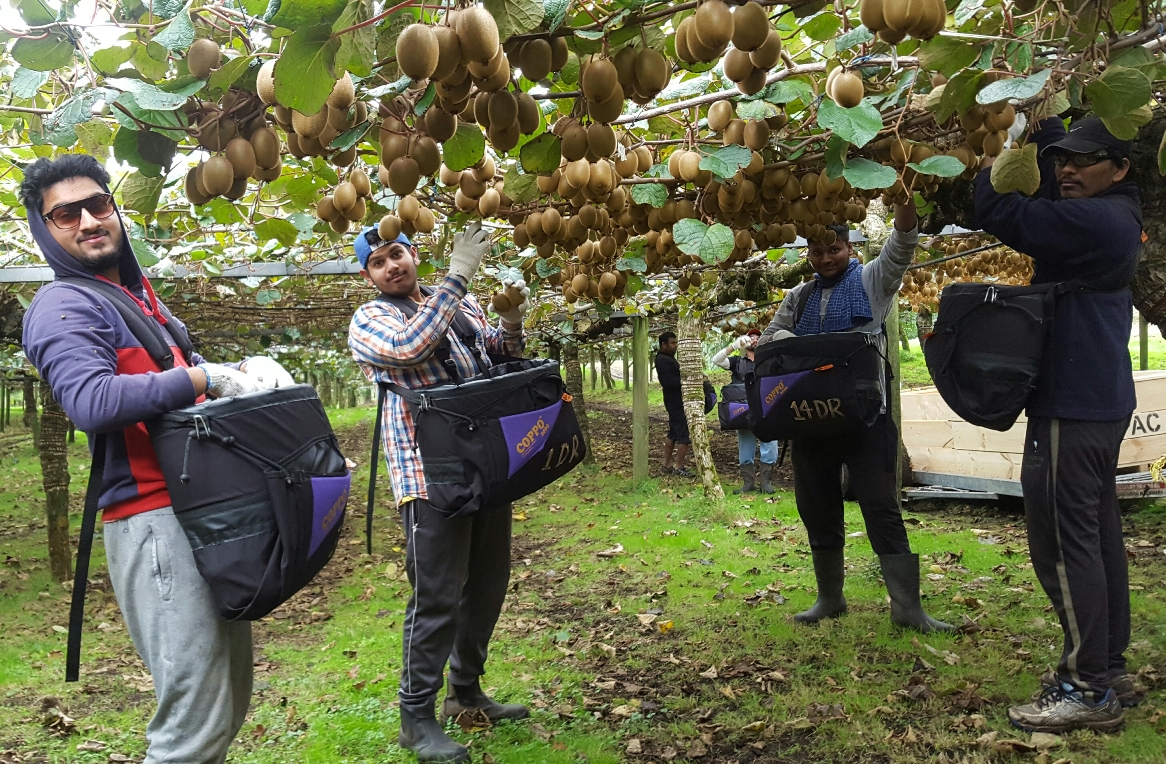
\includegraphics[scale=0.2]{Pickers}
\caption{Seasonal picking staff}
\label{fig:Picking}
\end{figure}

\section{Methodology}
\subsection{Research Scope}
Soft robotics is a revolutionary bio-inspired branch of robotics. It incorporates soft technologies which can potentially reduce the mechanical and algorithmic complexity in current robots. Soft technologies are. It allows robots to have bio-inspired capabilities such as flexible interactions in unpredictable environments \cite{kim2013soft}. The current autonomous methods of harvesting the fruits from the vine are very mechanical and often do not have the capability of harvesting the fruit delicately to ensure minimal or no bruising occurs to the specimen. Many of the handling mechanisms currently used grip the fruits too firmly, incorrectly, or do not morph around the shape of the specimen efficeintly, thus causing damage to the fruit. The most efficient of the current autonomous methods all have a biometric inspired design \cite{hassan2015design}. Thus it drawing inspiration from the shape of the humanoid hand, leading to optimal picking due to the fact that there are large amounts of surface area and force control. Bruising of fruits can cause the skin to split, leading to the opportunity for bacteria and fungi to enter the fruit. This causes the fruit to spoil at an accelerated rate, thus not being of an acceptable standard for purchase once it has made it to the point of retail.
\\
\newline
Considering the context of the problem which has been discussed above, research has been conducted into the current soft robotic grippers which could possibly be suitable to handle and manipulate delicate produce efficiently. The grippers which have been researched are as follows:
\begin{itemize}
\item Mechanically actuated
\item Tendon under actuated soft gripper
\item Pneumatic under actuated
\item Particle jamming 
\end{itemize}
Each of the above-mentioned methods have been thoroughly researched to determine their suitability by finding the advantages and disadvantages associated with each of the methods. From this research, it has been found that the most suitable method/mechanism is, in fact, the pneumatic under actuated method, however, it can still have improvements made to become more effective still. Thus, this method has been even further researched to look at the variations within the pneumatic field itself. Since up to date, the fruits have been predominantly been harvested by hand, biomimetric options have also been researched. The material composition of a soft robotic gripper greatly affects its functionality, optimal materials have also been researched.
\\
\newline
In order to have completed the required research to the highest possible standard, it was imperative to ensure that the resources which are being used are of the highest possible quality. In order to achieve this only resources which full filled the following requirements were used:
\begin{itemize}
\item Reputable Resources: Only articles which have been reviewed and previously cited by multiple other sources have been used.
\item Current Resources: All of the resources used were published no longer than 7 years ago. This means that the information discussed in the article is still relevant. The only exception for this was made for researching mechanical grippers due to the fact that it is an outdated model.
\end{itemize}
\section{Past and current Methods}
Soft robotic devices based on highly flaxable materials have gained a huge amount of traction and interest in the last decade due to their favourable characteristics such as compactness and ease of manufacturability \cite{mutlu2013electroactive}. There a wide range of grippers currently in the marketplace which have the potential to handle delicate produce such as fresh fruit and produce to various extents. Each of the viable options has been discussed below along with the advantages and disadvantages associated with each respective design.
\subsection{Mechanical}
Mechanical grippers were the first of the robotic grippers produced. They are produced using rigid links, mechanical joints as well as being actuated using a combination of linear actuators, pneumatic actuators and motors \cite{marchese2015recipe}. Mechanical grippers are very useful when high precision and rapid actuation is required, however, their shortcomings are quickly exposed when it comes to handling soft or delicate objects \cite{ilievski2011soft}. Due to this mechanical nature where rigid links and joints are required for actuation, mechanical grippers are heavy, costly, difficult to control and un-compliant to an array of different shapes \cite{martinez2014soft}. In order to make the mechanical gripper more compliant to delicate objects or irregular shapes, a wide range of sensors is required such as machine vision, tactile sensors, and switches. Without all of these sensors, the mechanical grippers are unable to determine how firm their grip is, thus often causing damage to the object being held, especially if the object is delicate \cite{ceccarelli2000designing}.
\\
\newline
The rigid materials used in production makes it very difficult to develop a mechanical gripper which is capable of handling a range of shapes without causing damage through point loading without the use of a very sophisticated sensor and control system. In the case of the two fingered design which is shown in Figure \ref{fig:Mechanical1}, it is clear to see that the gripper would not be fit for purpose Due to the minimal surface area over which the force will be spread, it is almost certain that the produce will be blemished or bruised. However, this design was produced in 1999 and since then huge improvements have been made even in the case of the mechanical grippers. 
\\
\newline
Figure \ref{fig:Mechanical2} is a concept for an apple picking robot which was developed in 2013. In order to make the gripper more compliant than traditional mechanical grippers, soft foam rubber was placed on each of the 4 fingers in order to provide cushioning and to distribute the pressure of the grip over a larger area \cite{chiu2013development}.When considering this mechanical gripper, there are still a number of issues which hinder its success when handling delicate produce which is outlined below:
\begin{itemize}
\item Point Loading: Even though there is cushioning in the touch interface, there is still limited degrees of freedom which can be used to conform around the objects. This means that there will be points where stress will be concentrated, leading to the potential for damage to the payload, especially of it is delicate like produce.
\item Control system: Order to know if an object has been gripped and the force exerted in that grip, numerous sensors are required \cite{chiu2013development}
\item Difficult control: The control of the mechanically actuated gripper is fairly difficult due to the numerous individual motors are actuation sources which are required to handle and manipulate objects \cite{marchese2015recipe}
\item Uncompliant: The gripper can only move into positions where its rigid geometry fits in due to the  fact that it has no flexibility.
\item Heavy: Due to all of the components required to actuate the gripper, causes it to be unnecessarily heavy and bulky.
\end{itemize}
From the research which has been done into the mechanically actuated grippers, it has become clear that they are not suitable to solve the  problem in the context of this research project. 
\begin{figure}[h]
\centering
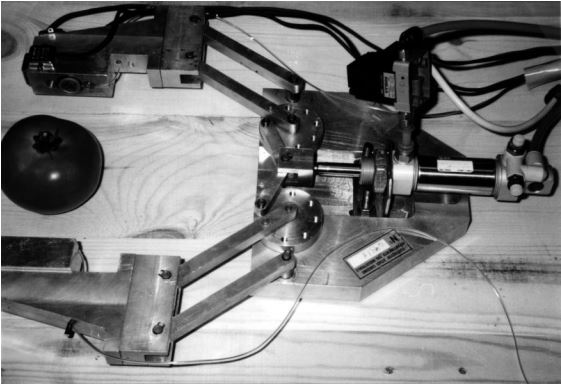
\includegraphics[scale=0.6]{Mechanical1}
\caption{Two Fingered Mechanical Gripper}
\label{fig:Mechanical1}
\end{figure}

\begin{figure}[h]
\centering
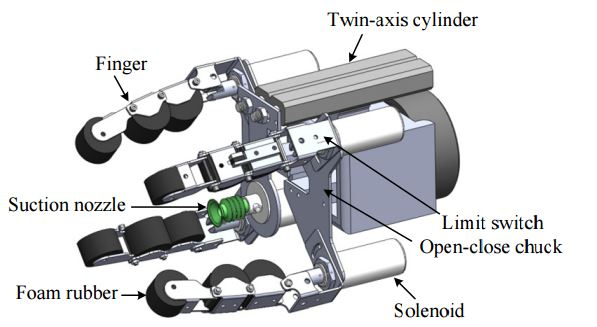
\includegraphics[scale=0.6]{Mechanical2}
\caption{Tomato Picking Mechanical Gripper}
\label{fig:Mechanical2}
\end{figure}

\subsection{Tendon actuated soft gripper}
Tendon actuated soft grippers were one of the first major leaps into the soft robotics field. The gripper is actuated using cables which are drawn mechanically using a combination of servo and linear actuators in order to achieve the desired range of motion \cite{marchese2015recipe}. The cables are usually composed of nylon-coated stainless steel, allowing them to be durable, sufficiently strong and able to pass through low friction tubing easily \cite{dollar2010contact}. The cable is anchored in a distal link in the tip of the finger then passes through the fingers of the gripper, usually through low friction tubing, to the respective source of actuation \cite{dollar2010contact}, which allows the joints of the finger to bend in relation to to the tension the cable as illustrated in Figure \ref{fig:Tendon}. The tendons are placeed off center, closer to the inside edge off desired actuation as shown in Figure \ref{fig:Tendon2}, thus once the cables are placed under tension, the finger will bend to the least restricted orientation, providing the grasping effect. In order to mimic the biological counterpart, which is a humanoid hand, the finger of the actuator should either be produced using rigid links which are encased in a compliant material or have a semi-rigid backbone \cite{mutlu2016mechanical}. Both of the methods have advantages and disadvantages depending on the application of the gripper, thus each gripper is discussed below in the context of this project
\subsubsection{Rigid Link Tendon Actuated}
By using a rigid link in the fingers of the gripper, it means that there is a limited amount of conformation which can occur. Depending on the application of the gripper this can be either an advantageous or disadvantageous trait. If the objects which are to be picked up are rigid and do not deform under relatively low pressures, then the rigid links would be advantageous. For the scope of this project where the gripper is intended to grip delicate produce such as kiwifruit, this style of gripper would not be very advantageous because it would cause point loading to an extent.

\subsubsection{Semi-Rigid Tendon Actuated}
Due to the fact that grippers are being developed to be more universal, more of the developers choose to make use of the second option of using a semi-rigid backbone. This allows for a greater amount of conformation to occur, resulting in a more compliant grip \cite{marchese2015recipe}. The semi-rigid material used in the production of this model is chosen such that it is capable of conforming about the object which it is gripping whilst still being able to support its own body weight and the weight of its payload \cite{hassan2015design}.

\subsubsection{Material Selection}
Since soft robotics often suffer from not being capable of carrying their own body weight \cite{mutlu2016mechanical}, it is important to select the material used in the production of the semi-rigid model to ensure that the materials allow the gripper to work as required. The grip interface should be produced using a very soft material to maximise surface area due to deformation upon applying force, however, the backbone should be stiff enough such that it is capable of impressing sufficient force onto the object being handled as well as sustaining its own weight \cite{hassan2015design}. In the case of the Under-Actuated Soft Gripper shown in Figure \ref{fig:Tendon2}, Dragon Skin 30 is used as the material for the touch interface due to the finish of the elastomer providing a good grip, low cost and having a low density \cite{hassan2015design}. The backbone of the gripper has been produced using Smooth-Sil 950 due to its Elastic modulus of 5MPa which allows the gripper to have enough rigidity to be able to support itself without hindering its grasping capabilities. The 3D Printed Soft Prosthetic Finger has used a similar but different approach. The designer has opted to use FilaFlex, a commercially available thermoplastic to produce the gripper. The FilaFlex was chosen due to the fact that it is low cost, 3D printable as well as being compliant \cite{mutlu2016mechanical}. By using a 3D printable thermoplastic, alterations of the  concept is made easier and more cost effective.
\begin{figure}[!h]
\centering
\begin{minipage}[b]{.55\textwidth}
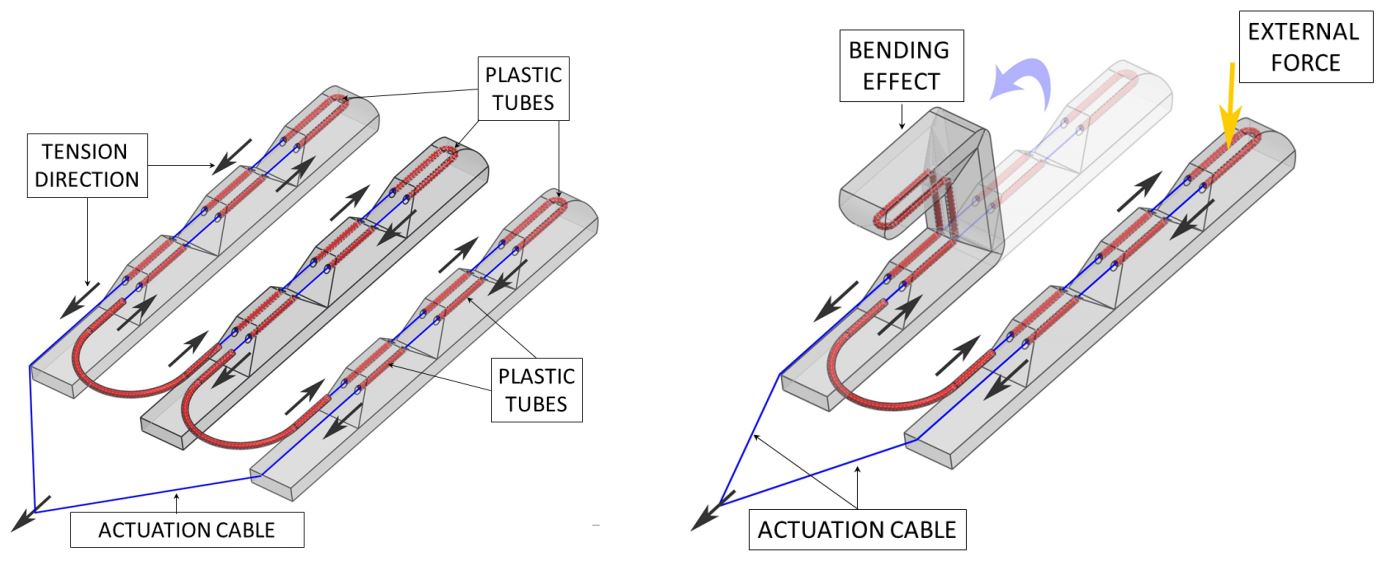
\includegraphics[width=\linewidth]{Tendon}
\caption{Under-Actuated Soft Gripper}
\label{fig:Tendon}
\end{minipage}
\hfill
\begin{minipage}[b]{0.35\textwidth}
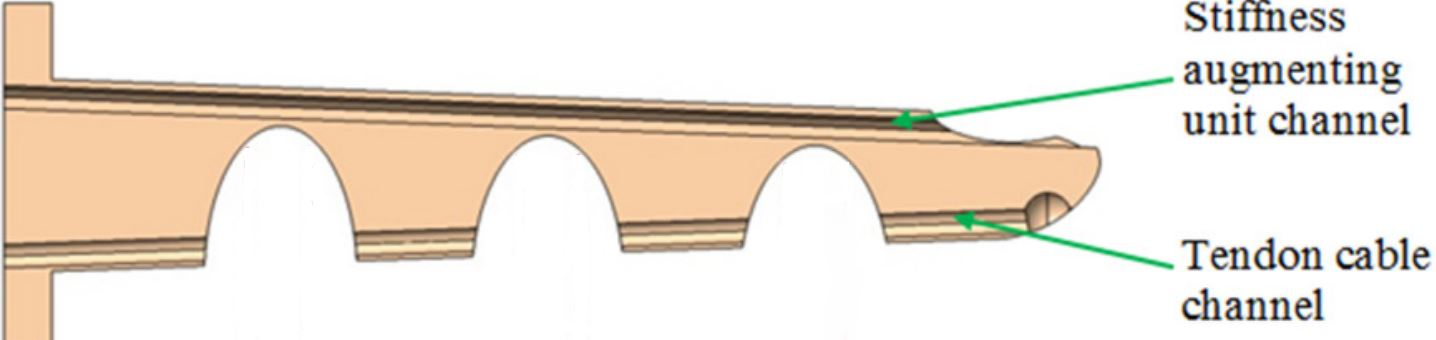
\includegraphics[width=1.15\linewidth]{Tendon2}
\caption{3D Printed Soft Prosthetic Finger}
\label{fig:Tendon2}
\end{minipage}
\end{figure}
\\
From the two Tendon actuated grippers which have been discussed above, it is clear to see that the semi-rigid gripper would be better suited to this project in comparison with the rigid bodied actuator. Provided the correct material selection, the semi-rigid gripper has the capability to carry its own body weight as well as the weight of the specified payload, whilst giving the opportunity for maximum conformation around the object being handled. By using the tendon actuated system, it has allowed the gripper to not only have its soft elastomer touch interface to conform around the target object but has also given the opportunity for the finger to bend at the joints to physically grasp the object, much like a human does. The simplicity of actuation is also a very attractive quality since all of the fingers can be actuated simultaneously using one motor or each finger can be actuated independently. The simplicity allows for an overall gripper which is relatively low cost, light and easy to control.
\subsection{Pneumatic under-actuated}
\begin{figure}[!h]
\centering
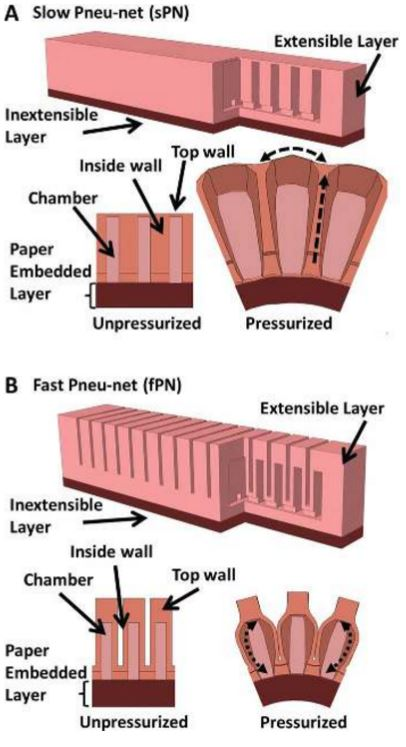
\includegraphics[scale=0.65]{Pneumatic1}
\caption{Soft Pneumatic Actuator.}
\label{pneumatic1}
\end{figure}
\noindent
The term underactuated describes universal grippers falling somewhere between active and passive distinctions \cite{amend2012positive}. Pneumatic grippers are soft robotics actuated by inflating specially designed elastomeric pockets called "pneu-nets", which are appealing for handling delicate and complex objects safely and securely whilst using very simple control \cite{mosadegh2014pneumatic}. In order to allow for actuation to occur, the pneu-nets which are the small channels embedded in the elastomer, are inflated at low pressure, usually 50 KPa, causing an increase of the internal volume of approximately 20 times \cite{mosadegh2014pneumatic}. By inflating the chambers, the pneu-nets expand and press against one another, causing the finger to be deflected to the side which does not have the pneu-nets located on it called the inextensable side \cite{ilievski2011soft}-\cite{marchese2015recipe}. By reducing the pressure in the pneu-nets below atmospheric pressure, a contraction in the pneu-net chambers is caused, thus causing the finger to deflect towards the extensable side of the actuator\cite{ilievski2011soft}-\cite{marchese2015recipe}.
\\
\newline
Pressurised air was used to actuate the gripper rather than using a hydraulic medium for due to the following advantages provided by using air \cite{mosadegh2014pneumatic}:
\begin{itemize}
\item Air provides rapid inflation due to its low viscosity.
\item Air is easily controlled and measured.
\item Air is available basically everywhere at no cost.
\item Air is light weight, thus does not put added strain on the actuator.
\item Air can be discarded after use by venting the air back into the atmosphere.
\item Air is compressible
\\
\newline
\end{itemize}
The performance of the Pneumatic Gripper depends on the layout of the Pneu-Nets. It is possible to make Pneumatic grippers which have very different capabilities and responses by making small alterations to the structure of the air chambers. As shown in Figure \ref{pneumatic1}, by having a small gap separating the individual pneumatic chambers, it gives the actuator the ability to actuate more rapidly due to the fact that there is a larger surface area for when actuating in the negative pressure sense, and internal pressure required to actuate in the positive sense is lower \cite{mosadegh2014pneumatic}.
\subsubsection{Pneu-Net configurations}
\begin{figure}[h]
\centering
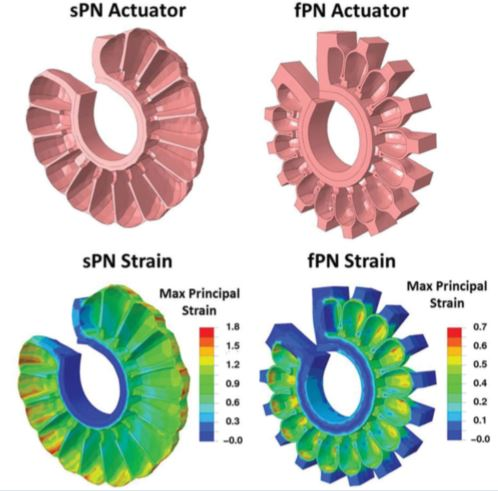
\includegraphics[scale=0.65]{Pneumatic2}
\caption{Developments in Pneu-Net actuation}
\label{fig:Pneumatic2}
\end{figure}
\subsubsection{Material Selection}
It is the compliance of the required of the materials used in the production of the pneu-nets that contribute to the greatest weakness of the pneumatic gripper \cite{shepherd2011multigait}. The weaknesses include:
\begin{itemize}
\item Slow actuation
\item Large change in volume
\item Short Lifespan
\end{itemize}
The slow actuation of the pneu-net can be altered if the actuator is designed such that the chambers are in the configuration explained in the fast pneu-net configuration. In order to allow the pneu-nets to expand, the gripper needs to be produced using a material which has a low enough modulus of elasticity to allow each of the chambers to expand reasonably easily. It is imperative that the pneu-net chambers are only capable of expanding on one side of the actuator, otherwise, the actuators will not work.
\newline
\begin{table}[!h]
\caption{Materials for production of soft pneumatic actuators}
\label{Pneumatic_table}
\centering
\begin{tabular}{ |p{4cm}|p{4cm}| }
 \hline
 \multicolumn{2}{|c|}{\textbf{Materials Used in Production}} \\
 \hline
 \textbf{Extensive side} & \textbf{In-extensive Side}\\
 \hline
 EcoFlex 0300 \cite{ilievski2011soft},\cite{bilodeau2015monolithic},\cite{mosadegh2014pneumatic}   & Silgard 184 (PDMS)  \cite{ilievski2011soft},\cite{bilodeau2015monolithic} \\
 Dragon Skin \cite{hao2016universal} &   Elastosil M4601 \cite{mosadegh2014pneumatic}\\
 & Dragon Skin \cite{hao2016universal}\\
 \hline
\end{tabular}
\end{table}
\\
\newline
There is a definite trend in the materials which have been used as shown in table \ref{Pneumatic_table}. The Pneu-Net side of the actuator is often produced using EcoFlex 0300 due to its relatively low Young's modulus of elasticity of approximately 0.1 MPa. This modulus allows the Pneu-net chambers to contract and expand with relatively low loss of energy. The extensive side has a bit more variation in materials which are used. The modulus of elasticity for the extensive materials tends to range from approximately 5 to 7 Mpa. This allows the actuator to bend according to the state of the status of the Pneu-Nets whilst still having the rigidity to support its own weight and the weight of the object being handled as shown in Figure \ref{gripped}.
\begin{figure}[!h]
\centering
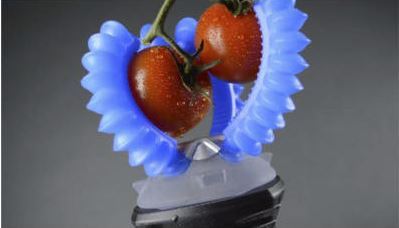
\includegraphics[scale=0.65]{gripped}
\caption{Pneumatic gripper grasping delicate produce}
\label{gripped}
\end{figure}
\subsection{Particle jamming}
\begin{figure}[!h]
\centering
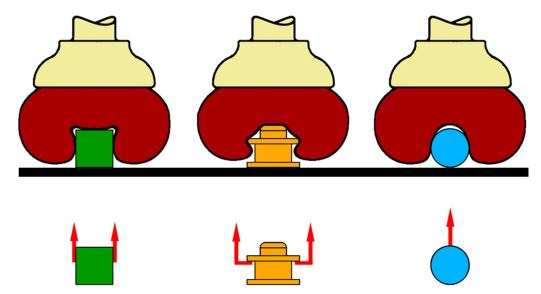
\includegraphics[scale=0.65]{jammer1}
\caption{Particle Jammer}
\label{jammer1}
\end{figure}
\noindent
Particle jamming is a novel method of manipulating and handling irregular and difficult to handle shapes. The working basis of the particle jammer is that it makes use of the following key aspects to perform easy and effective grasping \cite{amend2012positive}:
\begin{itemize}
\item Static friction from surface contact.
\item Geometric constraints from the captured target object through interlocking.
\item Vacuum suction when an airtight seal is achieved on some portion of the object's interface.  
\end{itemize}
The conventional universal grippers are capable of both grasping and manipulation but also engender extensive physical and computational complexity, which is evident in the grasp algorithm research \cite{miller2003automatic},\cite{shimoga1996robot},\cite{saxena2008robotic}. Due to the complexities evolved with the traditional universal grippers, coupled with their correspondingly high costs, have limited their adoption among commercial robotic industries \cite{amend2012positive}.

\begin{figure}[h]
\centering
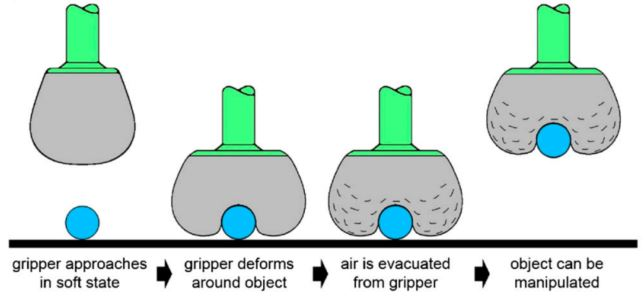
\includegraphics[scale=0.6]{jammer2}
\caption{Operation of a particle jammer}
\label{fig:jammer2}
\end{figure}
\subsubsection{Materials and makeup}
The working principals of the particle jammer is very simple since the only machinery needed to actuate the gripper is a vacuum pump. In order to make the gripper fully autonomous, a positive displacement pneumatic pump is also required \cite{amend2012positive}. Optimal performance is observed if the gripper is returned back to the "neutral" position after each "grab". This is done by loosening the granules in the gripper after each grip either manually by kneading and shaking the gripper or mechanically by giving the gripper a pulse of positive pressure in the latex sac to free the granules \cite{amend2012positive}. If the granules are not reset back to the neutral position, the ability to grip object rapidly decreases with each grip. A working particle jammer thus required the following materials to operate\cite{amend2012positive}:
\begin{enumerate}
\item Positive displacement pump
\item Vacuum pump
\item Fine granular medium
\item Latex sac/balloon
\item Housing/mount
\end{enumerate}
\subsubsection{Operating }
The operation of the granular operator is illustrated in Figure \ref{fig:Pneumatic2}. The steps to hold onto a target object the following steps need to occur:
\begin{enumerate}
\item Reset the gripper to neutral position: As mentioned before, this can be done manually by shaking the gripper and kneading the latex balloon. However since the gripper is supposed to be able to work autonomously, it is better to reset the granules by subjecting the granules to a positive pressure impulse of air.
\item Move the gripper into a position where it is over the target object such that the object is protruding into the gripper by approximately 1cm.
\item Evacuate the air in the latex bag: The desired gripping action is produced at this stage through a combination of 3 effects:
\begin{itemize}
\item Friction: The friction force results from slight (< 0.5\%) volume contraction of the latex membrane causing the membrane to pinch onto the target object causing a frictional force to be normal to the point of contact \cite{amend2012positive}, \cite{brown2010universal}.
\item Interlocking: When the volume of the latex membrane reduces due to the air in the membrane being removed, often the granular material will interlock around the geometry of the target object \cite{brown2010universal}.
\item Vacuum suction on the object surface: If an air tight seal is made on a portion of the target geometry, a suction force is produced.
\end{itemize} 
\item Move the gripper to the desired location
\item Release the object: In order to release the object, the pressure in the latex membrane has to simply be restored back atmospheric pressure.
\item Repeat steps 1-5 as required.  
\end{enumerate}
The gripper based on the principle of jamming granular material tend to be able to successfully grasp any object provided the gripper membrane can sufficiently reach around the sides of the object being held to create a large enough pinching force \cite{brown2010universal}. 
\section{Electroactive Polymer}
Electroactive polymers are a distinguished class of polymeric materials with the unique ability to change shape and size upon activation from an electrical current \cite{pillay2014review}. The actuator is actuated depending on the orientation of the electro-active layers and the electrical charge on each respective layer. When an electrical input is applied to PPy(Polypyrole) layer, it stimulates counter-ions to` move in and out of the PPy layers. While the positively charged layer is oxidised, the negatively charged polymer layer is consequently reduced. The anions move from the electrolyte to the positively charged PPy layer, thus the opposite effect is observed by the negatively charged PPy layer. The resultant ion transfer causes a volume expansion in the positively charged layer and a contraction in the negatively charged layer \cite{mutlu2013electroactive}. This process is what allows the actuation of the system to occur. Reversing the process will actuate the system in the reverse direction.
\\
\newline
The response time and performance in terms of actuation force produced can be changed depending on the electroactive polymer which is used and the voltage which is applied. However, regardless of the materials used, this method of gripping is suited for "micro actuation" due to the fact that the forces which can be produced are so small\cite{bogue2016flexible}. One major drawback which limits the use of the electropolymerization is the small yield of polymer since the electropolymerisation process only occurs on the surface of the electrodes \cite{pillay2014review}. Since the force is directly proportional to the surface are of the PPy layer, thus, in order to have sufficient force to produce a successful grasp, a huge amount of surface are will be required. When considering this fact, it becomes clear that this method of gripping is not suitable for the context of this project.
\begin{figure}[h]
\centering
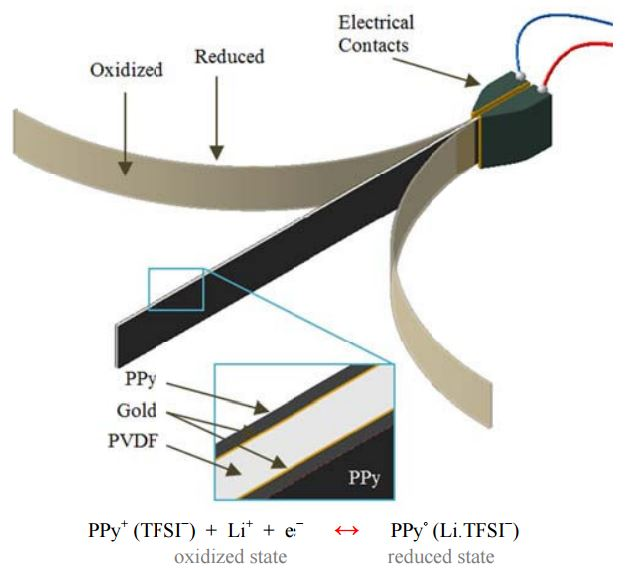
\includegraphics[scale=0.6]{electroactive}
\caption{Operation of an eleactroactive actuator}
\label{fig:electro1}
\end{figure}
\section{Current Trends }
From the analysis which has been done on each n the current options, it was prominent to see that the most promising of the methods was indeed the pneumatically actuated model. This model has been testing using a wide range of configurations and
The material used to produce a compliment soft robotic gripper is very important due to the fact that the material used can completely change the performance of the gripper. In th
\section{Conclusion}
The capability to handle delicate and fragile goods autonomously using robotics has been long sought after, thus, in the preceding report, a range of popular gripping methods have been explored and investigated. The research has been done to find a range of robotic and soft robotic grippers to deduce which methods or aspects of each respective method could be used as inspiration towards solving the context of this research problem. Soft robotics is defined as a subset of robotics in which the machines are built using compliant materials with variable stiffness actuators and compliant control \cite{wolf2008actively}.
\\
\newline
The kiwifruit industry in New Zealand is worth in excess of \$1,181.9 billion dollars \cite{fresh_facts_2015}, yet virtually all of the harvesting of the produce is completed manually by a seasonal workforce. Due to the physical requirements of the of the harvesting process, the work does take a great physical toll on the workers who have to carry the produce from the place where it has been picked to the transportation carts as well as pick all of the produce from a position which is elevated above their heads. This physical stress to which the workers are subjected to do often cause injury to the workers, thus contributing to the \$7,283,868 worth in ACC claims to treat people whom have injured themselves by lifting heavy objects in farming situations \cite{injury_statistics_tool_2017}. Due to the injuries which is often experienced by farm workers, it means that the farmers have to pay ever increasing ACC levies, ultimately driving the cost of the produce up and leading to loss of revenue in terms of exports for the local economy.
\\
\newline
A range of different gripping methods was explored during the course of the preceding literature review and it was found that some methods are more suitable for the desired application of picking delicate fruit and berries than others. The methods which were researched are:
\begin{itemize}
\item Mechanical Gripper
\item Tendon Actuated soft gripper
\item Pneumatic under actuated gripper
\item Particle jamming gripper
\item Electro Active Polymers
\end{itemize}
In the context of this research problem, the current trends in the industry suggest that the most suitable of the investigated methods are in fact the Pneumatic under actuated gripper and possibly the tendon actuated soft gripper. Due to the compliance, simple control and ease of manufacture of the pneumatic under-actuated gripper, it seems to be the most suitable of all of the respective gripping methods. The mechanical gripper is simply and outdated method which is heavy, bulky and expensive to manufacture, ruling it to be redundant for the given application. The particle jammer often makes use of interlocking with the geometry of the object which is to be grasped, jet in order to make use of the particle jammer, the physical gripper would have the be too large to make it applicable. As for the electroactive polymer gripper, the forces which are created in actuation would not be sufficient to conform around the  fruit as well as having enough force to pick the fruit from the vine, thus, causing it the unsuitable for the problem at hand at this stage.
\\
\newline
The research which has been done is to be used as a guide for the project in order to develop and deduce the optimal gripping method for the purpose of gripping delicate fruits and berries. The choice as to which gripper will be used is not final, as further research will be done during the course of the 228.798 Individual Research Paper
\bibliographystyle{ieeetr}
\bibliography{Reference}
\end{document}